\documentclass{beamer}

% Theme selection (you can experiment with different themes)
\usetheme{Madrid}
\usepackage[backend=biber]{biblatex}
\addbibresource{references.bib} % A clean and commonly used theme
% \usetheme{Warsaw} % Another popular choice
% \usetheme{CambridgeUS} % More minimalist

% Color themes (optional, can be used with specific themes)
% \usecolortheme{beaver}
% \usecolortheme{dolphin}

% Font setup (optional, if you want different fonts)
% \usepackage{lmodern} % Latin Modern font
% \usepackage{amsmath} % For mathematical equations if needed

\usepackage{graphicx} % Required for including images (your logo)
% ADD THIS LINE FOR AUTOMATIC FIGURE NUMBERING
\setbeamertemplate{caption}[numbered]
% Unicode fixes
\usepackage[utf8]{inputenc}
\usepackage[T1]{fontenc}
\DeclareUnicodeCharacter{2013}{--}   % en-dash
\DeclareUnicodeCharacter{2014}{---}  % em-dash
\DeclareUnicodeCharacter{201C}{``}   % left double quote
\DeclareUnicodeCharacter{201D}{''}   % right double quote
\DeclareUnicodeCharacter{00A0}{ }    % non-breaking space
\DeclareUnicodeCharacter{03BB}{\Lambda} % Greek Lambda
\DeclareUnicodeCharacter{00B0}{\degree} % Degree symbol
\DeclareUnicodeCharacter{2192}{$\rightarrow$} % arrow
\DeclareUnicodeCharacter{039B}{$\Lambda$}


%----------------------------------------------------------------------------------------
%   TITLE PAGE
%----------------------------------------------------------------------------------------

\title{An Optimal Energy Absorption and Utilization Design for Deformable/Reconfigurable Modular Solar-Powered UAVs in Near Space
}

\author{VISMAYA K (LWYD22EE073)}
\institute{S7 B.Tech EEE \\ Guided by: Prof. MUHAMMED RAFI (Assistant Professor, EEE Dept.) \\ Government Engineering College, Wayanad}
\date{October 13, 2025}

% Add the logo to the title page specifically at the bottom center
\titlegraphic{%
	\vfill % Push everything above to the top
	\centering % Center the logo horizontally
	
\includegraphics[height=1.5cm]{cropped-logo.png} % Replace with your logo file and adjust size
	\vfill % Push the logo to the bottom
}

\begin{document}
	
	% Title page frame
	\begin{frame}
		\titlepage
	\end{frame}
	\begin{frame}
		\frametitle{Outline}
		\tableofcontents
	\end{frame}
	
	%----------------------------------------------------------------------------------------
%   SECTION SLIDES
%----------------------------------------------------------------------------------------

\section{INTRODUCTION}
\begin{frame}{INTRODUCTION}
    \framesubtitle{
}
    \begin{itemize}
        \item Global issues like climate change and energy shortage demand sustainable aviation solutions.  
        \item Solar-powered UAVs (SP-UAVs) can achieve long-endurance, low-cost, and flexible flight operations.  
        \item Conventional fossil-fuel and battery-powered aircraft are limited in endurance.  
        \item Challenges exist in solar energy absorption and energy storage efficiency.  
        \item Deformable and reconfigurable modular UAVs enhance solar utilization and mission performance.  
    \end{itemize}
\end{frame}

\section{MOTIVATION AND OBJECTIVES}
\begin{frame}{MOTIVATION AND OBJECTIVES}
    \textbf{Motivation}
    \begin{itemize}
        \item Growing demand for clean and sustainable aviation solutions.
        \item Need for long-endurance platforms for surveillance, communication, and disaster management.
        \item Limitations of conventional fossil-fuel and battery-powered aircraft.
        \item Potential of solar-powered UAVs to provide near-permanent flight.
        \item Opportunity to enhance performance using deformable and reconfigurable modular designs.
    \end{itemize}
    
    \vspace{0.3cm}
    
    \textbf{Objectives}
    \begin{itemize}
        \item Design an efficient solar-powered UAV platform.
        \item Maximize solar energy absorption and utilization.
        \item Reduce structural weight while maintaining payload.
        \item Improve endurance and mission adaptability.
        \item Develop an optimization framework for sustainable flight.
    \end{itemize}
\end{frame}
\section{LITERATURE SURVEY}
\begin{frame}{LITERATURE SURVEY}
    \framesubtitle{}
    \begin{table}[]
        \centering
        \scriptsize % Reduce font size to fit content better
        \begin{tabular}{|p{2.8cm}|p{2.8cm}|p{4.8cm}|}
            \hline
            \textbf{Reference} & \textbf{Focus Area} & \textbf{Key Findings / Contributions} \\ \hline
            Youngblood et al. (1984) & Early solar aircraft design & Proposed design methodology integrating solar and fuel cell propulsion for long endurance. \\ \hline
            Noth (2008) & Analytical design frameworks & Developed subsystem models and analytical tools for continuous solar-powered flight. \\ \hline
            Aurora Flight Sciences (2007) & Morphing (Odysseus concept) & Introduced Z-shaped wing configuration to maximize solar absorption. \\ \hline
            Wu et al. (2017–2019) & Sun-tracking / morphing UAVs & Investigated Z-shaped, N-shaped, and 3-shaped wings for improved energy capture and endurance. \\ \hline
            Montalvo \& Castello (2015), Magill (2002) & Reconfigurable / meta-aircraft & Explored wingtip connection and docking concepts, showing 20–40\% aerodynamic performance improvement. \\ \hline
            Wang et al. (2020, 2022) & Mission-oriented path planning & Proposed 3D path optimization with ant colony and cooperative energy optimization for modular UAVs. \\ \hline
            Gao et al. (2014), Li et al. (2020) & Battery and propulsion optimization & Highlighted importance of gravity energy storage, propulsion-focused design, and battery mass minimization. \\ \hline
        \end{tabular}
    \end{table}
\end{frame}

	
	\section{RELATED WORK}
\begin{frame}{RELATED WORK}
    \framesubtitle{Solar-Powered UAV Development}
    \begin{itemize}
        \item \textbf{Youngblood et al. (1984)}: Pioneered solar aircraft design methodology integrating solar and fuel cell propulsion
        \item \textbf{Noth (2008)}: Developed analytical frameworks and subsystem models for continuous solar-powered flight
        \item \textbf{Aurora Flight Sciences (2007)}: Introduced Odysseus concept with Z-shaped wing for maximum solar absorption
        \item \textbf{Wu et al. (2017-2019)}: Investigated Z-shaped, N-shaped, and Λ-shaped wings for improved energy capture
        \item \textbf{Montalvo \& Costello (2015)}: Proposed meta-aircraft concept with wingtip connection
        \item \textbf{Magill (2002)}: Showed 20-40\% aerodynamic improvement through wingtip docking
        \item \textbf{Wang et al. (2020, 2022)}: Developed mission-oriented 3D path planning with energy optimization
    \end{itemize}
\end{frame}

% Page 1
\begin{frame}{SYSTEM MODELING}
    \framesubtitle{Mass, Aerodynamic, and Energy Models}
    
    \begin{block}{Mass Prediction Model}
    \begin{equation*}
        m_{total} = m_{struc} + m_{batt} + m_{sc} + m_{mppt} + m_{prop} + m_{fixed}
    \end{equation*}
    \end{block}
    
    \begin{block}{Aerodynamic Model}
    \begin{equation*}
        C_D = C_{D0} + C_{Dp} + \frac{C_L^2}{\pi eAR}
    \end{equation*}
    \end{block}
    
    \vspace{-0.2cm}
    \begin{block}{Energy Balance}
    \begin{equation*}
        \int_{24h} P_{absorb}dt \geq \int_{24h} P_{consume}dt
    \end{equation*}
    \end{block}
    
    \vspace{-0.2cm}
    \begin{block}{Solar Radiation Model}
    \begin{equation*}
        P_{sc} = \sum_i^n (\eta_{sc} SI_h \cos(\mathbf{n_s}, \mathbf{n_{sc}}) S)_i
    \end{equation*}
    \end{block}
\end{frame}

\section{DEFORMABLE/RECONFIGURABLE CONCEPT}

% Page 1: Main concept with image
\begin{frame}{DEFORMABLE/RECONFIGURABLE CONCEPT}
    \framesubtitle{Innovative Platform Design}
    \begin{figure}
        \centering
        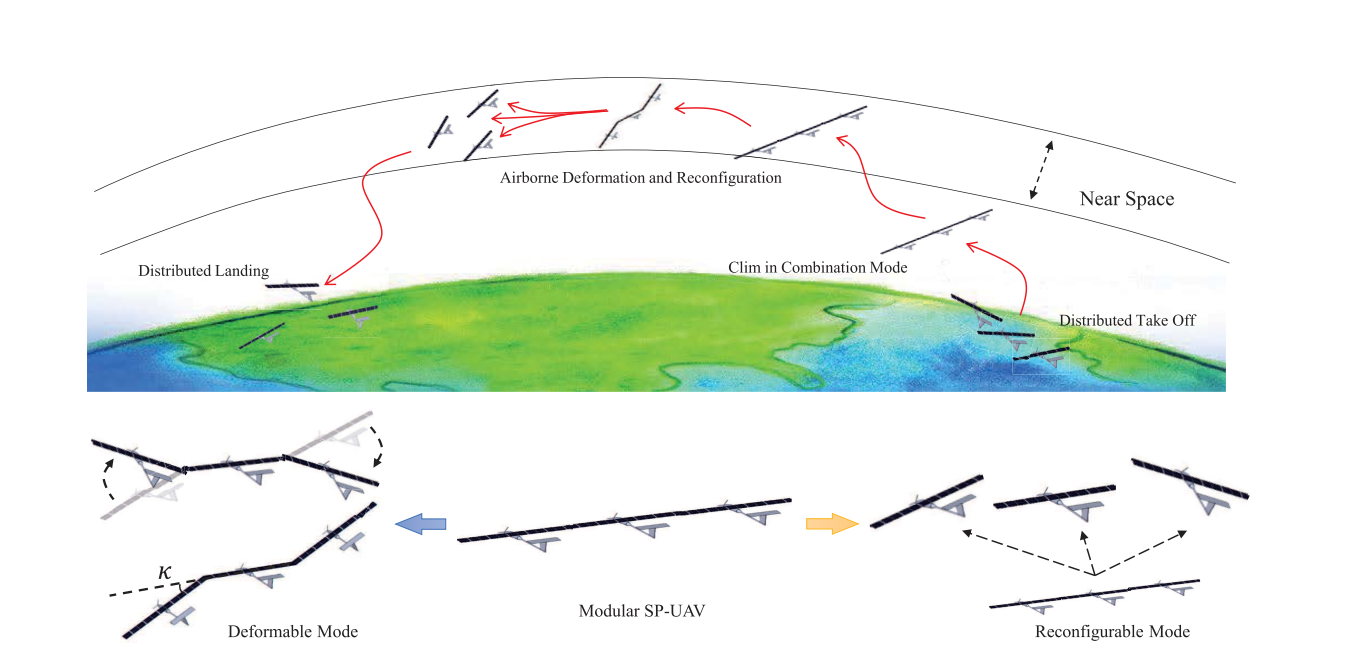
\includegraphics[width=0.7\textwidth]{concept.png}
        \caption{Concept for a deformable/reconfigurable SP-UAV}
        \label{fig:deformable_concept}
    \end{figure}
    
    \begin{itemize}
        \item \textbf{Deformable SP-UAV:} Wings adjust dihedral angle for optimal solar absorption
        \item \textbf{Reconfigurable SP-UAV:} Multiple aircraft connect/disconnect for mission flexibility
    \end{itemize}
\end{frame}

% Page 2: Deformable SP-UAV - Technical Details & Benefits
\begin{frame}{DEFORMABLE SP-UAV}
    \framesubtitle{Adaptive Wing Configuration \& Performance}
    
    \textbf{Key Features:}
    \begin{itemize}
        \item Outer wings deform upward/downward
        \item Dihedral angle range: $\kappa \in [-30^\circ, 30^\circ]$
        \item Adaptive control: $\kappa = \min(\kappa_{max}, 90^\circ - \alpha)$
        \item Real-time optimization based on solar position
    \end{itemize}
    
    \vspace{0.3cm}
    \textbf{Operational Strategy:}
    \begin{itemize}
        \item \textbf{Day:} Adjust wings to maximize solar absorption
        \item \textbf{Night:} Maintain flat configuration for aerodynamics
    \end{itemize}
    
    \vspace{0.3cm}
    \textbf{Performance Benefits:}
    \begin{itemize}
        \item Increased solar energy capture during daylight
        \item Improved aerodynamic efficiency at night
        \item Extended mission endurance
    \end{itemize}
    
    \begin{alertblock}{Key Improvement}
        17.2\% mass reduction compared to conventional design
    \end{alertblock}
\end{frame}

% Page 3: Reconfigurable SP-UAV - Architecture & Energy Management
\begin{frame}{RECONFIGURABLE SP-UAV}
    \framesubtitle{Modular Architecture \& Energy Management}
    
    \textbf{Configuration Modes:}
    \begin{itemize}
        \item \textbf{Combined Mode:}
        \begin{itemize}
            \item Single entity operation
            \item Energy conservation during night
            \item Reduced power consumption
        \end{itemize}
        \item \textbf{Separated Mode:}
        \begin{itemize}
            \item Independent operation
            \item Multiple simultaneous missions
            \item Increased coverage area
        \end{itemize}
    \end{itemize}
    
    \vspace{0.3cm}
    \textbf{Energy Constraints:}
    \begin{itemize}
        \item Real-time: $P_{consume}(t) \leq P_{absorb}(t)$
        \item Daily: $\int_{24h} P_{consume}dt \leq \int_{24h} P_{absorb}dt$
    \end{itemize}
    
    \vspace{0.3cm}
    \begin{alertblock}{System Benefit}
        97\% increase in feasible mission days
    \end{alertblock}
\end{frame}

\section{FLIGHT STRATEGY}

% First page - Image only
\begin{frame}{FLIGHT STRATEGY}
    \framesubtitle{Optimal Energy Management}
    
    \begin{figure}
        \centering
        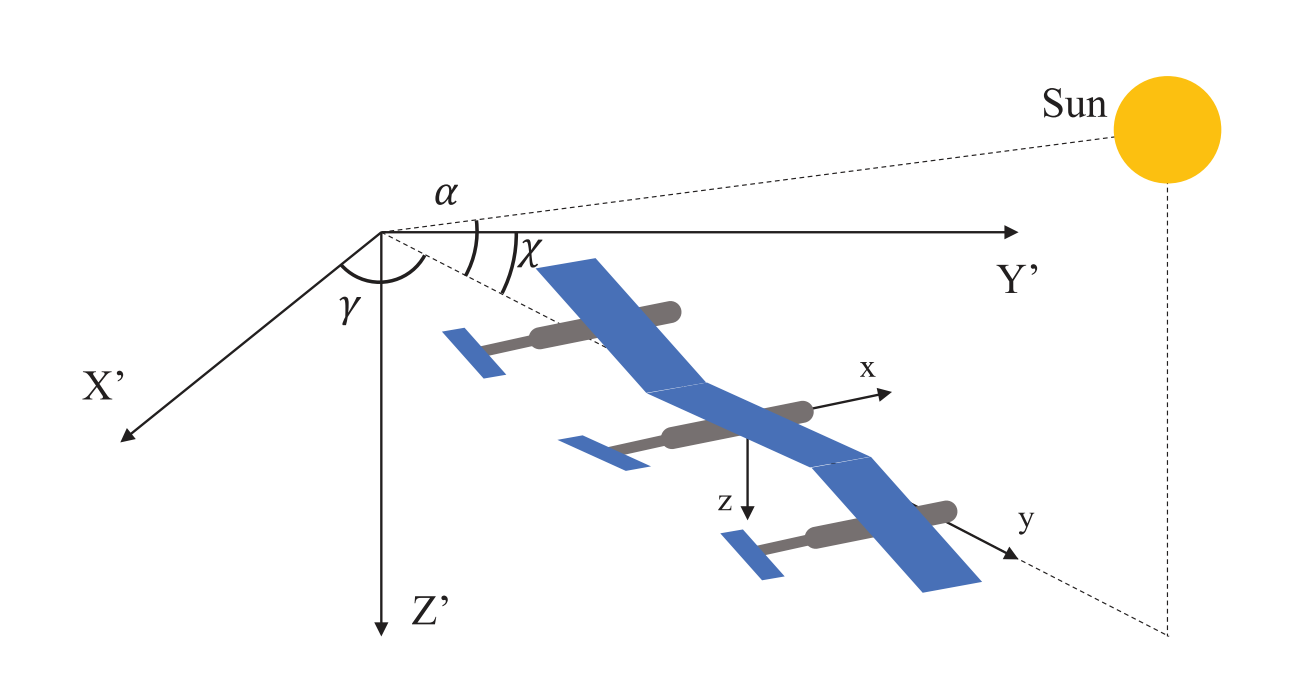
\includegraphics[width=0.9\textwidth]{flight_strategy.png}
        \caption{Flight profile of reconfigurable SP-UAV showing separation and combination points}
        \label{fig:flight_strategy}
    \end{figure}
\end{frame}

% Second page - Key Constraints
\begin{frame}{FLIGHT STRATEGY}
    \framesubtitle{Energy Balance Constraints}
    
    \textbf{Key Constraints:}
    \begin{equation*}
        \begin{cases}
            P_{consume}(t_1) \leq P_{absorb}(t_1) \\
            \int_{24h} P_{consume}dt \leq \int_{24h} P_{absorb}dt
        \end{cases}
    \end{equation*}
    
    \vspace{0.5cm}
    \textbf{Constraint Explanation:}
    \begin{itemize}
        \item \textbf{Real-time constraint:} Instantaneous power consumption must not exceed absorption
        \item \textbf{Daily constraint:} Total daily energy consumption must not exceed total absorption
        \item Ensures continuous operation without energy depletion
        \item Guides separation/combination timing decisions
    \end{itemize}
    
    \vspace{0.3cm}
    \textbf{Application:}
    \begin{itemize}
        \item Determines when to separate into individual units
        \item Controls when to combine for energy conservation
        \item Optimizes mission duration and coverage
    \end{itemize}
\end{frame}

\section{OPTIMIZATION FRAMEWORK}

% Page 1: Diagram only
\begin{frame}{OPTIMIZATION FRAMEWORK}
    \framesubtitle{Overall Optimization Process}
    \begin{figure}
        \centering
        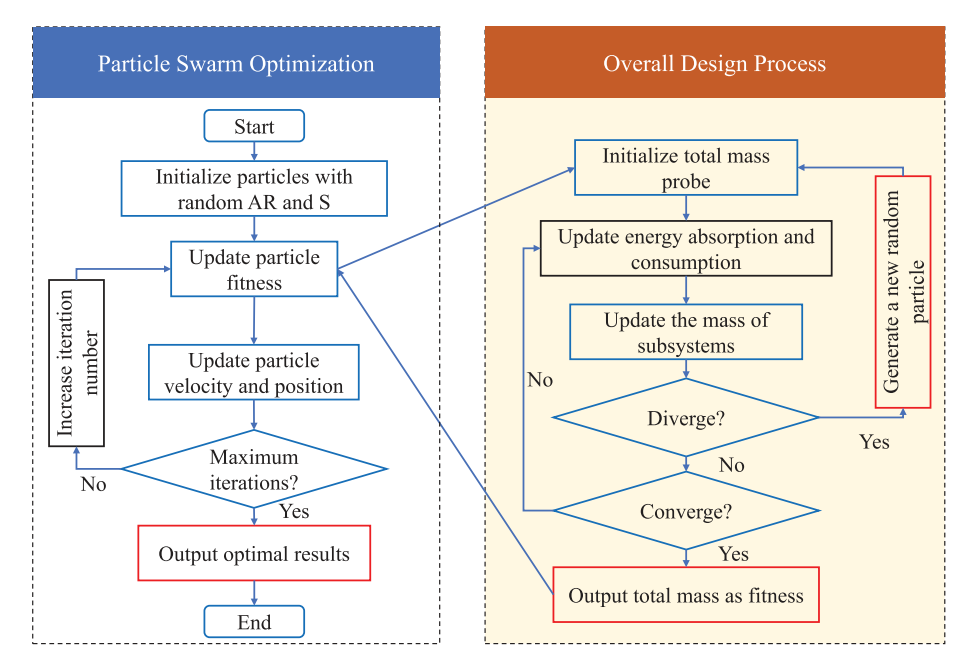
\includegraphics[width=0.8\textwidth]{optimation_framework.png} % Reduced from 0.9
        \caption{Particle Swarm Optimization Framework}
        \label{fig:optimization_framework}
    \end{figure}
\end{frame}

% Page 2: PSO Algorithm Details
\begin{frame}{OPTIMIZATION FRAMEWORK}
    \framesubtitle{Particle Swarm Optimization (PSO) Algorithm}
    
    \textbf{Objective Function:}
    \begin{equation*}
        \min: m_{total} \quad \text{subject to:} \quad b_{min} < b < b_{max}, \quad S_{min} < S < S_{max}
    \end{equation*}
    
    \textbf{PSO Update Equations:}
    \begin{align*}
        V_i^{k+1} &= \omega V_i^k + c_1 r_1 (P_i^k - X_i^k) + c_2 r_2 (P_g^k - X_i^k) \\
        X_i^{k+1} &= X_i^k + V_i^{k+1}
    \end{align*}
    
    \textbf{Algorithm Parameters:}
    \begin{itemize}
        \item $\omega$: Inertia weight (controls momentum)
        \item $c_1, c_2$: Cognitive and social acceleration coefficients
        \item $r_1, r_2$: Random numbers uniformly distributed in [0,1]
        \item $P_i^k$: Personal best position of particle $i$
        \item $P_g^k$: Global best position in the swarm
    \end{itemize}
\end{frame}

% Page 3: Design Variables and Process
\begin{frame}{OPTIMIZATION FRAMEWORK}
    \framesubtitle{Design Variables and Optimization Process}
    
    \textbf{Design Variables:}
    \begin{itemize}
        \item Reference area ($S_{ref}$) - Wing surface area
        \item Aspect ratio (AR) - Ratio of wingspan to chord length
        \item Optimized for minimum total weight while maintaining performance
    \end{itemize}
    
    \vspace{0.3cm}
    \textbf{Optimization Process Features:}
    \begin{itemize}
        \item Population-based stochastic optimization
        \item Particles represent potential design solutions
        \item Fitness evaluation based on mass minimization
        \item Constraint handling for energy balance
        \item Convergence to global optimum through swarm intelligence
    \end{itemize}
    
    \vspace{0.3cm}
    \textbf{Key Advantages:}
    \begin{itemize}
        \item Handles non-linear design spaces effectively
        \item Robust convergence characteristics
        \item Suitable for multi-variable optimization problems
    \end{itemize}
\end{frame}

\section{OVERALL DESIGN PROCESS} 
\begin{frame}{OVERALL DESIGN PROCESS}
    \framesubtitle{Iterative Mass and Energy Balance}
    
    \begin{figure}
        \centering
        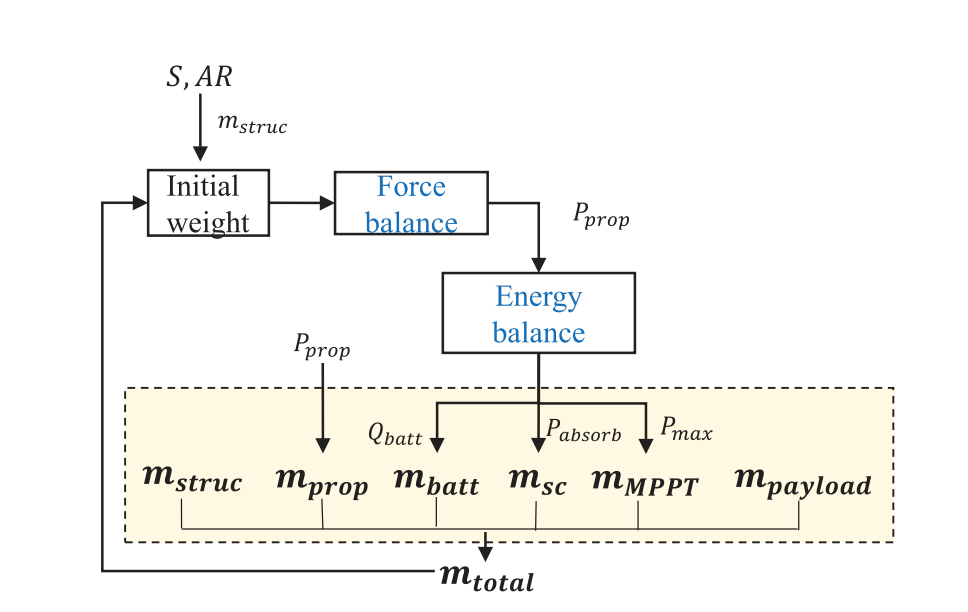
\includegraphics[width=0.85\textwidth]{design_process.png}
        \caption{Overall parameter selection and optimization flow}
    \end{figure}
    
    \begin{itemize}
        \item Initial weight estimation from structural mass (41.2\% of total)
        \item Iterative update of subsystem masses
        \item Convergence check for total mass
        \item Energy balance validation
    \end{itemize}
\end{frame}

\section{RESULTS AND ANALYSIS}
\begin{frame}{OPTIMIZATION RESULTS}
    \framesubtitle{Performance Comparison}
    
    \begin{table}
        \centering
        \begin{tabular}{|l|c|c|c|}
            \hline
            \textbf{Parameter} & \textbf{Planar} & \textbf{Deformable} & \textbf{Change} \\
            \hline
            Total mass (kg) & 1224.2 & 1013.8 & -17.2\% \\
            Reference area (m²) & 285.2 & 219.1 & -23.2\% \\
            Aspect ratio & 29.6 & 29.6 & - \\
            \hline
        \end{tabular}
        \caption{Optimal design results comparison}
    \end{table}
    
    \textbf{Key Improvements:}
    \begin{itemize}
        \item 17.2\% reduction in total mass
        \item 23.2\% reduction in reference area
        \item Same aspect ratio maintained
        \item Payload remains constant at 50 kg
    \end{itemize}
\end{frame}

\section{ENERGY PERFORMANCE} 
% First page - Images only
\begin{frame}{ENERGY PERFORMANCE}
    \framesubtitle{Solar Absorption and Battery Management}
    
    \begin{columns}
        \begin{column}{0.5\textwidth}
            \begin{figure}
                \centering
                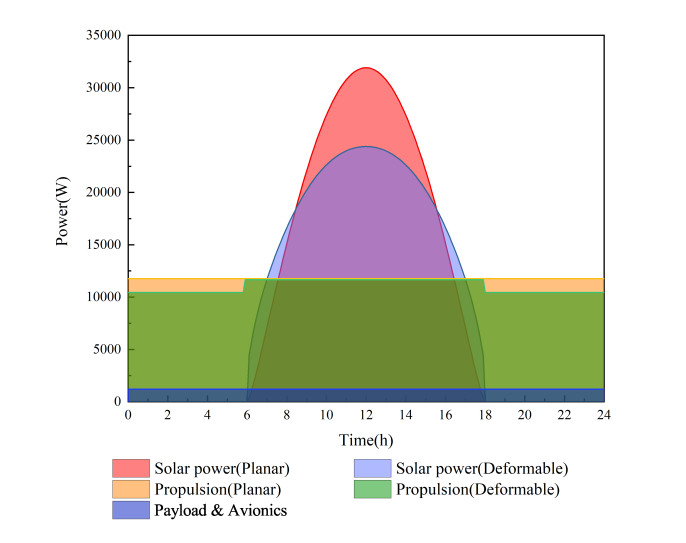
\includegraphics[width=\textwidth]{power_curve.png}
                \caption{Power absorption and consumption}
            \end{figure}
        \end{column}
        \begin{column}{0.5\textwidth}
            \begin{figure}
                \centering
                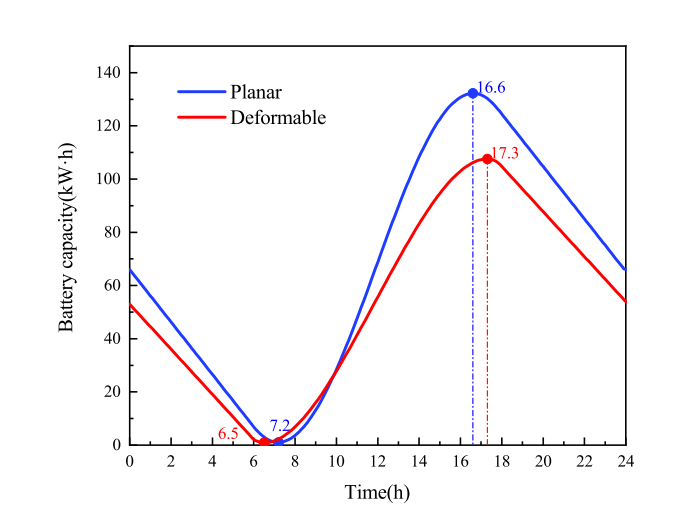
\includegraphics[width=\textwidth]{soc_curve.png}
                \caption{Battery state of charge}
            \end{figure}
        \end{column}
    \end{columns}
\end{frame}

% Second page - Analysis points
\begin{frame}{ENERGY PERFORMANCE}
    \framesubtitle{Performance Analysis}
    
    \textbf{Key Improvements:}
    \begin{itemize}
        \item Extended equivalent daytime period
        \item Reduced battery discharge duration (14.6h → 13.2h)
        \item Faster battery recharge during daylight
        \item Improved energy utilization efficiency
        \item Enhanced power management system
    \end{itemize}
    
    \vspace{0.5cm}
    \textbf{Impact on Mission Performance:}
    \begin{itemize}
        \item Longer operational endurance
        \item Increased mission reliability
        \item Better adaptation to varying solar conditions
        \item Optimized energy storage utilization
    \end{itemize}
\end{frame}

\section{MISSION PERFORMANCE} 
\begin{frame}{MISSION PERFORMANCE}
    \framesubtitle{Feasible Operation Analysis}
    
    \begin{table}
        \centering
        \begin{tabular}{|l|c|c|c|}
            \hline
            \textbf{Configuration} & \textbf{Left Boundary} & \textbf{Right Boundary} & \textbf{Days} \\
            \hline
            Deformable & April 11th & September 1st & 142 \\
            Planar & May 15th & July 25th & 72 \\
            \hline
        \end{tabular}
        \caption{Feasible mission duration comparison}
    \end{table}
    
    \textbf{Performance Gains:}
    \begin{itemize}
        \item 97\% increase in feasible mission days (72 → 142 days)
        \item Wider operational latitude and date range
        \item Enhanced mission adaptability
    \end{itemize}
    
    \textbf{Case Study:} Urumqi to Haikou (3408 km) mission feasibility
\end{frame}

\section{PARAMETER SENSITIVITY} 
% First page - Images only
\begin{frame}{PARAMETER SENSITIVITY}
    \framesubtitle{System Parameter Effects}
    
    \begin{columns}
        \begin{column}{0.5\textwidth}
            \begin{figure}
                \centering
                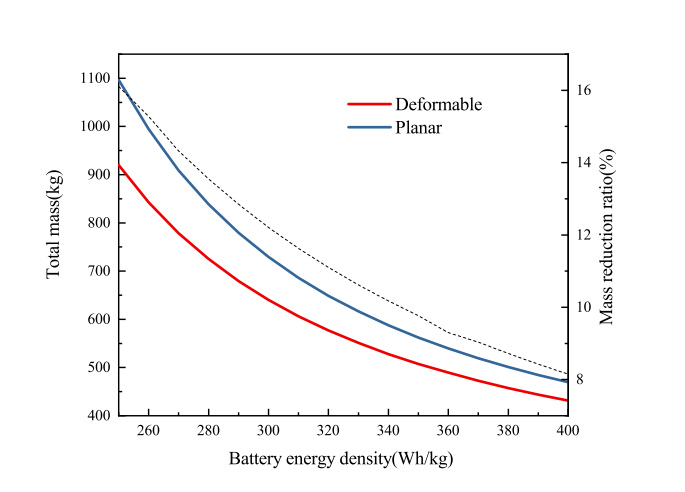
\includegraphics[width=\textwidth]{battery_sensitivity.png}
                \caption{Effect of battery energy density}
            \end{figure}
        \end{column}
        \begin{column}{0.5\textwidth}
            \begin{figure}
                \centering
                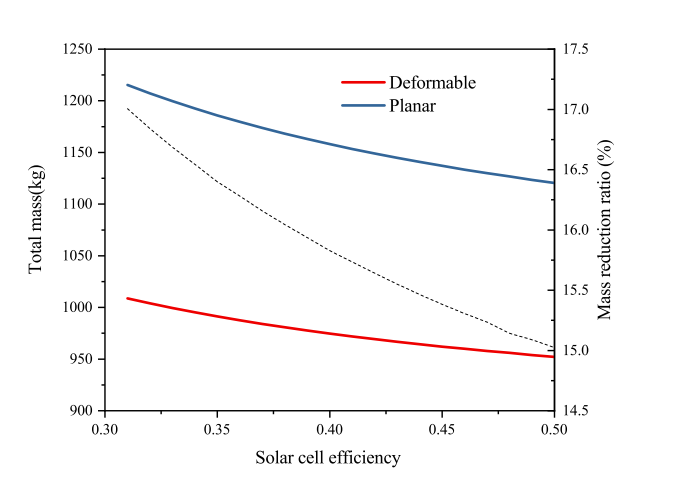
\includegraphics[width=\textwidth]{solar_sensitivity.png}
                \caption{Effect of solar cell efficiency}
            \end{figure}
        \end{column}
    \end{columns}
\end{frame}

% Second page - Analysis points
\begin{frame}{PARAMETER SENSITIVITY}
    \framesubtitle{Sensitivity Analysis Results}
    
    \textbf{Key Findings:}
    \begin{itemize}
        \item Battery density: 240-400 Wh/kg reduces mass by ~50\%
        \item Solar efficiency: 0.3-0.5 provides moderate mass reduction
        \item Optimal aspect ratio around 30 for both configurations
        \item Battery technology has highest impact on system mass
        \item Solar cell efficiency shows diminishing returns above 0.4
    \end{itemize}
    
    \vspace{0.5cm}
    \textbf{Design Implications:}
    \begin{itemize}
        \item Focus on battery technology advancement for maximum benefit
        \item Target solar efficiency in the 0.35-0.45 range for cost-effectiveness
        \item Maintain aspect ratio near 30 for optimal performance
        \item Balance trade-offs between different subsystem improvements
    \end{itemize}
\end{frame}

\section{CONCLUSION}
\begin{frame}{CONCLUSION}
    \framesubtitle{Key Contributions and Findings}
    
    \textbf{Main Achievements:}
    \begin{itemize}
        \item Developed innovative deformable/reconfigurable SP-UAV platform
        \item Proposed integrated design methodology with PSO optimization
        \item Achieved 17.2\% mass reduction compared to conventional design
        \item Extended feasible mission duration from 72 to 142 days (97\% increase)
        \item Enhanced energy utilization through adaptive wing morphing
    \end{itemize}
    
    \textbf{Technical Innovations:}
    \begin{itemize}
        \item Joint optimization of energy absorption and mission utility
        \item Comprehensive modeling of mass, aerodynamics, and energy systems
        \item Adaptive flight strategies for different solar conditions
        \item Modular architecture enabling multiple mission profiles
    \end{itemize}
\end{frame}

\begin{frame}{FUTURE WORK}
    \framesubtitle{Potential Extensions and Improvements}
    
    \begin{itemize}
        \item Investigate asymmetrical wing parts or subunits
        \item Explore multiple flight profiles and mission scenarios
        \item Develop advanced control strategies for morphing aircraft
        \item Integrate weather prediction for adaptive mission planning
        \item Study thermal effects on solar cell efficiency at high altitudes
        \item Investigate hybrid energy storage systems
        \item Develop real-time optimization algorithms for dynamic environments
    \end{itemize}
\end{frame}
\section{REFERENCES}

% Page 1 of References
\begin{frame}{References}
    \scriptsize
    \setlength{\itemsep}{1pt}
    \setlength{\parskip}{1pt}
    \begin{thebibliography}{99}
        
        \bibitem{ref1} Z. Li et al., ``An Optimal Energy Absorption and Utilization Design for Deformable/Reconfigurable Modular Solar-Powered UAVs,'' \emph{IEEE Access}, vol. 10, pp. 91948-91962, 2022.
        
        \bibitem{ref2} J. Youngblood et al., ``Design of long-endurance unmanned airplanes,'' in \emph{Proc. 20th Joint Propuls. Conf.}, 1984.
        
        \bibitem{ref3} A. Noth, ``Design of solar powered airplanes for continuous flight,'' Ph.D. dissertation, ETH Zurich, 2008.
        
        \bibitem{ref4} X.-Z. Gao et al., ``Joint optimization of battery mass and flight trajectory,'' \emph{Proc. Inst. Mech. Eng., G. J. Aerosp. Eng.}, vol. 228, no. 13, pp. 2439-2451, 2014.
        
        \bibitem{ref5} X. Li et al., ``General optimal design of solar-powered UAV,'' \emph{Chin. J. Aeronaut.}, vol. 33, no. 8, pp. 2176-2188, 2020.
        
        \bibitem{ref6} M. Wu et al., ``Optimal flight planning for a Z-Shaped morphing-wing UAV,'' \emph{J. Guid., Control, Dyn.}, vol. 41, no. 2, pp. 497-505, 2018.
        
        \bibitem{ref7} M. Wu et al., ``Effect of solar cell efficiency on optimal flight control,'' \emph{Acta Astronautica}, vol. 164, pp. 366-375, 2019.
        
        \bibitem{ref8} C. Montalvo and M. Costello, ``Meta aircraft flight dynamics,'' \emph{J. Aircr.}, vol. 52, no. 1, pp. 107-115, 2015.
        
    \end{thebibliography}
\end{frame}

% Page 2 of References
\begin{frame}{References (Continued)}
    \scriptsize
    \setlength{\itemsep}{1pt}
    \setlength{\parskip}{1pt}
    \begin{thebibliography}{99}
        \setcounter{enumiv}{8} % Continue numbering from 9
        
        \bibitem{ref9} S. Magill, ``Compound aircraft transport,'' Ph.D. Dissertation, Virginia Tech, 2002.
        
        \bibitem{ref10} X. Wang et al., ``Mission-oriented cooperative 3D path planning,'' \emph{Chin. J. Aeronaut.}, vol. 35, no. 1, pp. 98-109, 2022.
        
        \bibitem{ref11} J. Kennedy and R. Eberhart, ``Particle swarm optimization,'' in \emph{Proc. IEEE ICNN}, vol. 4, 1995.
        
        \bibitem{ref12} P. Mardanpour and D. H. Hodges, ``Passive morphing of flying wing aircraft,'' \emph{J. Fluids Struct.}, vol. 44, pp. 17-30, 2014.
        
        \bibitem{ref13} M. Wu et al., ``Morphing wing solar-powered aircraft,'' \emph{J. Aircr.}, vol. 54, no. 5, pp. 1996-2002, 2017.
        
        \bibitem{ref14} M. Wu et al., ``A-shaped rotatable wing aircraft,'' \emph{Aerosp. Sci. Technol.}, vol. 98, 2020.
        
        \bibitem{ref15} X. Zhu et al., ``Solar-powered airplanes: A historical perspective,'' \emph{Prog. Aerosp. Sci.}, vol. 71, pp. 36-53, 2014.
        
    \end{thebibliography}
\end{frame}
% Minimalist Thank You page
\begin{frame}
    \centering
    \vspace{1.5cm}
    
    \Huge \textbf{Thank You}
    
    \vspace{1cm}
    \Large Questions?
\end{frame}
	
\end{document}
